\documentclass[10pt]{article}
\usepackage[polish]{babel}
\usepackage[utf8]{inputenc}
\usepackage[T1]{fontenc}
\usepackage{graphicx}
\usepackage[export]{adjustbox}
\graphicspath{ {./images/} }
\usepackage{amsmath}
\usepackage{amsfonts}
\usepackage{amssymb}
\usepackage[version=4]{mhchem}
\usepackage{stmaryrd}

\title{XI Konkurs matematyczny St@ś }

\author{}
\date{}


\begin{document}
\maketitle
XIV LO im. Stanisława Staszica\\
30 maja 2011 roku

\section*{klasa VI}
Na rozwiqzanie poniższych zadań masz 90 minut.\\
Kolejność rozwiazywania zadań jest dowolna.\\
Wszystkie zadania sa jednakowo punktowane.\\
Maksymalnq liczbę punktów może uzyskać jedynie petne rozwiqzanie, z uzasadnieniem i odpowiedziq.\\
Używanie korektora i korzystanie z kalkulatora jest niedozwolone.

\section*{Zadanie 1.}
Czy suma 2011 różnych liczb pierwszych może być liczbą parzystą?

\section*{Zadanie 2.}
Dane są liczby 1, 2, 3, 4, 5, 6 oraz sześcian, na ścianach którego trzeba wpisać wszystkie te liczby. Sumy liczb na przeciwległych ścianach muszą być równe.\\
Przerysuj siatkę sześcianu i na każdej ścianie napisz jedną z tych liczb.\\
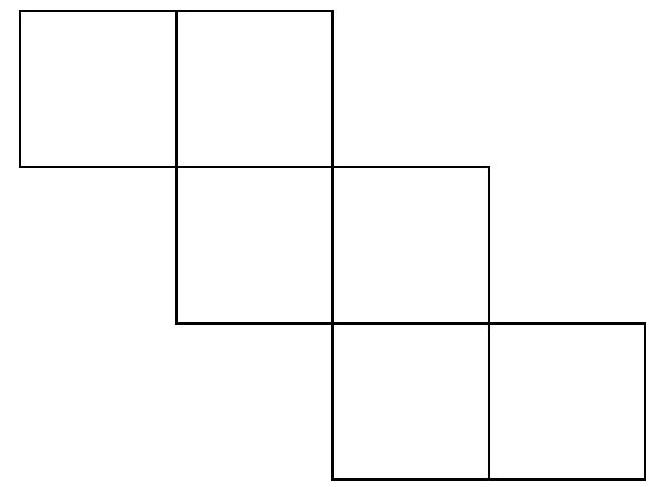
\includegraphics[max width=\textwidth, center]{2024_11_21_3799db89e062e92fb27eg-1}

\section*{Zadanie 3.}
Dany jest taki trójkąt \(A B C\), w którym miara każdego kąta wyraża się naturalną liczbą stopni. Kąt \(B A C\) jest 5 razy większy od kąta \(A B C\). Miara kąta \(B C A\) wyraża pewną liczbą stopni. Uzasadnij, że jest to liczba podzielna przez 6.

\section*{Zadanie 4.}
Dany jest romb \(A B C D\) o boku długości 1. Na boku \(C D\) leży taki punkt \(E\), że pole trójkąta \(A E D\) jest trzy razy mniejsze od pola czworokąta \(A B C E\). Oblicz długość odcinka \(C E\).

\section*{Zadanie 5.}
Niektóre liczby w dodawaniu ułamków zwykłych zasłonięto kartami. Wszystkie zasłonięte liczby są naturalne i dodatnie. Jaką liczbę zasłonięto szarą kartą? Ile rozwiązań ma to zadanie?\\
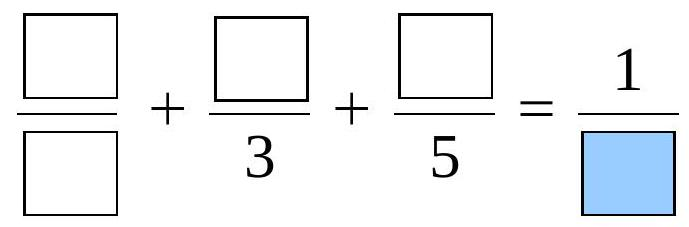
\includegraphics[max width=\textwidth, center]{2024_11_21_3799db89e062e92fb27eg-1(1)}


\end{document}